\documentclass{standalone}
\usepackage{pgfplots}
\pgfplotsset{compat=1.18}
\usepgfplotslibrary{colorbrewer}
\pgfplotsset{cycle list/Set1-6}

\begin{document}

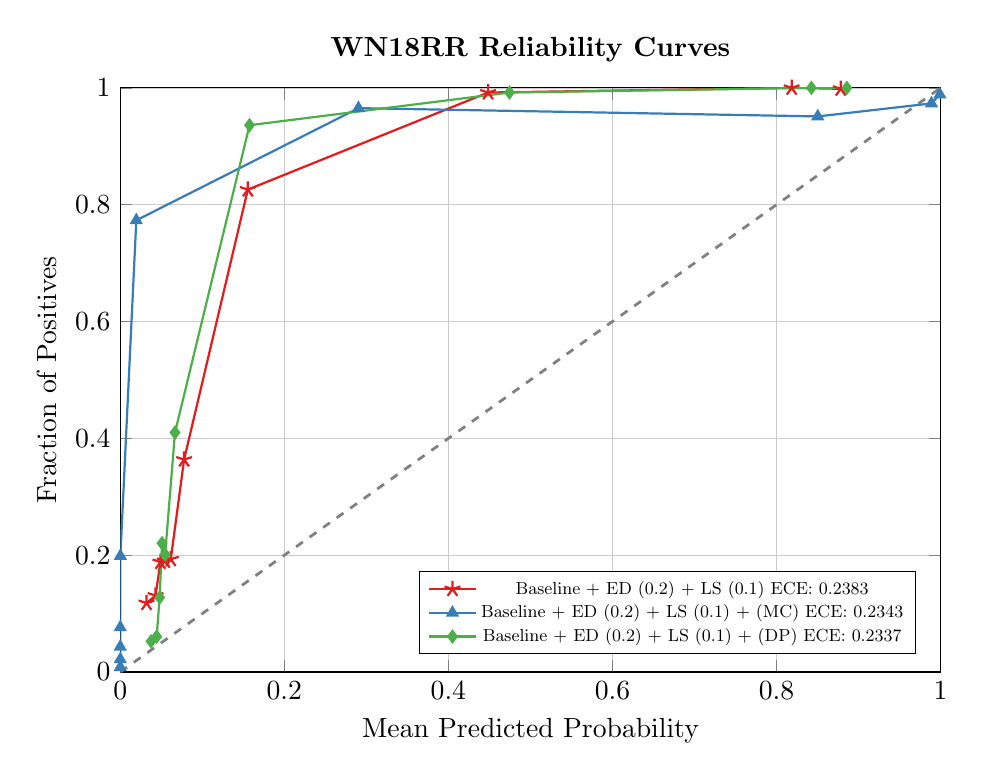
\begin{tikzpicture}
\begin{axis}[
    title={\textbf{WN18RR Reliability Curves}},
    xlabel={Mean Predicted Probability},
    ylabel={Fraction of Positives},
    xmin=0, xmax=1,
    ymin=0, ymax=1,
    xtick={0, 0.2, 0.4, 0.6, 0.8, 1.0},
    ytick={0, 0.2, 0.4, 0.6, 0.8, 1.0},
    legend pos= south east,
    legend style={nodes={scale=0.7, transform shape}, font=\small},
    grid=both,
    grid style={line width=.1pt, draw=gray!20},
    major grid style={line width=.2pt, draw=gray!40},
    width=12cm,
    height=9cm,
    cycle list name=Set1-6
]

% Perfectly Calibrated Line
\addplot [color=gray, dashed, line width=1pt, forget plot]
    coordinates {(0,0)(1,1)};

% Baseline + Edge Dropout (0.2) + Label Smoothing (0.1)
\addplot+[mark=star, thick, mark size=3pt] coordinates {
    (0.03203425, 0.11802233) (0.04300495, 0.1307815) (0.04899793, 0.18819777) (0.05433433, 0.19009585)
    (0.06158307, 0.19298246) (0.07781916, 0.36363636) (0.15551917, 0.82587859) (0.44843249, 0.99202552)
    (0.81844665, 1.0) (0.87824613, 0.9984051)
};
\addlegendentry{Baseline + ED (0.2) + LS (0.1) ECE: 0.2383}

\addplot+[mark=triangle*, thick] coordinates {
    (8.08637221e-11, 0.00830484) (1.27878564e-08, 0.02174444) (3.47365550e-07, 0.04324456) (5.52997593e-06, 0.07647203)
    (1.38037954e-04, 0.19863181) (1.95757910e-02, 0.77327144) (2.90354831e-01, 0.96530662) (8.50231506e-01, 0.95113609)
    (9.88813320e-01, 0.97336917) (9.99124482e-01, 0.98851979)
};
\addlegendentry{Baseline + ED (0.2) + LS (0.1) + (MC) ECE: 0.2343}

\addplot+[mark=diamond*, thick] coordinates {
    (0.03750767, 0.05263158) (0.04441421, 0.06060606) (0.04800265, 0.12759171) (0.05092608, 0.22044728)
    (0.05469451, 0.20095694) (0.06670213, 0.40988836) (0.15760037, 0.93610224) (0.47446698, 0.99202552)
    (0.8424876, 1.0) (0.88566874, 1.0)
};
\addlegendentry{Baseline + ED (0.2) + LS (0.1) + (DP) ECE: 0.2337}


\end{axis}
\end{tikzpicture}

\end{document}